\chapter{Teoretické východiská učiacich sa systémov na báze odmeňovania}

V tejto kapitole budú stručne predstavené učiace sa systémy založené na odmeňovaní.
Kapitola si kladie za cieľ ukázať princípy, matematické detaily budú
rozobraté v ďalšej kapitole.

\section{Úvod}

Strojové učenie predstavuje ďalší logický krok v počítačovej vede. Programovanie
založené na pevne danom správaní prestáva pre mnohé úlohy stačiť. Na softvérové
produkty sú kladené čoraz väčšie nároky, a v dohľadnej dobe sa dá očakávať
dosiahnutie hranice tradičného prístupu. Dôvodom je najmä veľmi rozsiahly stavový
priestor úloh. Možným východiskom sú adaptíve a učiace sa systémy.

Samotné učenie, alebo adaptácia, predstavuje zmenu parametrov systému.
V súčastnosti sú známe tri najpoužívanješie spôsoby učenia

\begin{enumerate}
\item minimalizácia chyby, ktorá je definovaná v každom kroku
\item vyhľadávanie podobných príznakov a zhluková analýza
\item odmeňovanie alebo trestanie vykonaných rozhodnutí
\end{enumerate}

{\bf Prvý spôsob} zahŕňa systémy učené na princípe predkladania dvojíc
vstup, požadovaný výstup. Učené sú napríklad metódou najmenších
štvorcov \cite{bib:adaptive_01} \cite{bib:adaptive_02} \cite{bib:adaptive_03},
alebo často používané gradientové metódy učenia neurónových sietí \cite{bib:gradient_01} \cite{bib:gradient_02}
\cite{bib:gradient_03} \cite{bib:backpropagation_00} \cite{bib:gradient_04}, prípadne
iteratívne učené regulátory \cite{bib:ilc_01} \cite{bib:ilc_02}, používané napr. v polohovacích mechanizmoch.
Sú to typické systémy učenia s učiteľom.

{\bf Druhý spôsob} je typický zástupca učenia bez učiteľa. Vstupy do systému
sú triedené podľa príznakov. Pobobné vstupy sú zatriedené do rovnakej skupiny.
Definícia podobnosti sa líši podľa aplikácie. Je to vlastne problém o zavedení vhodnej metriky
pre danú úlohu. Niekedy postačuje euklidova metrika, pre rôznorodé vlastnosti príznakov je často
potrebné ováhovať jednotlivé príznaky. Typickými zástupcami
sú Kohonenové siete \cite{bib:kohonen_01} \cite{bib:kohonen_02} \cite{bib:kohonen_03} ich špeciálny prípad je K-means.

{\bf Tretí spôsob} je použiteľný v situáciach, kedy je možné stanoviť rozdiel
výstupu a požadovaného výstupu len v niekoľkých prípadoch, pričom dosiahnutie
výstupu vyžaduje niekoľko krokov. Počas týchto krokov môžu byť systému
poskytované odmeny, na základe ktorých preohodnocuje svoje rozhodnutia.
Použiteľný je teda v situáciach, kde je potrebných viac krokov na dosiahnutie cieľa,
ale ich postupnosť nie je známa. To je podstatný rozdiel oproti napr.
iteratívne učenými regulátormi, kde sa síce tiež dosahuje požadovaná hodnota niekoľkými krokmi, avšak je v každom z nich známa
chyba oproti požadovanému správaniu.
Práve tejto kategórií je venovaná dizertačná práca.

{\bf Hybridné hierarchické systémy} predstavujú kombináciu niekoľkých princípov.
V prípade riadenie, je obvykle dynamika stroja známa - je možné stanoviť jeho fyzikálny model,
prípadne použiť adaptívny systém (je možné ukázať, že pre množstvo mechanických sústav je PID
regulátor vyhovujúce riešenie). Samotný blok riadenia regulátorom však nevypovedá o žiadanej hodnote -
snaží sa na ňu systém dostať, ale nevie ju stanoviť. V jednoduchých situáciach to nepredstavuje problém.

Pre komplexné riadnie je nevyhnutné systém rozdeliť do niekoľkých vrstiev, obrázok \ref{img:hierachical_controll_system}.

\begin{figure}[!htb]
\center
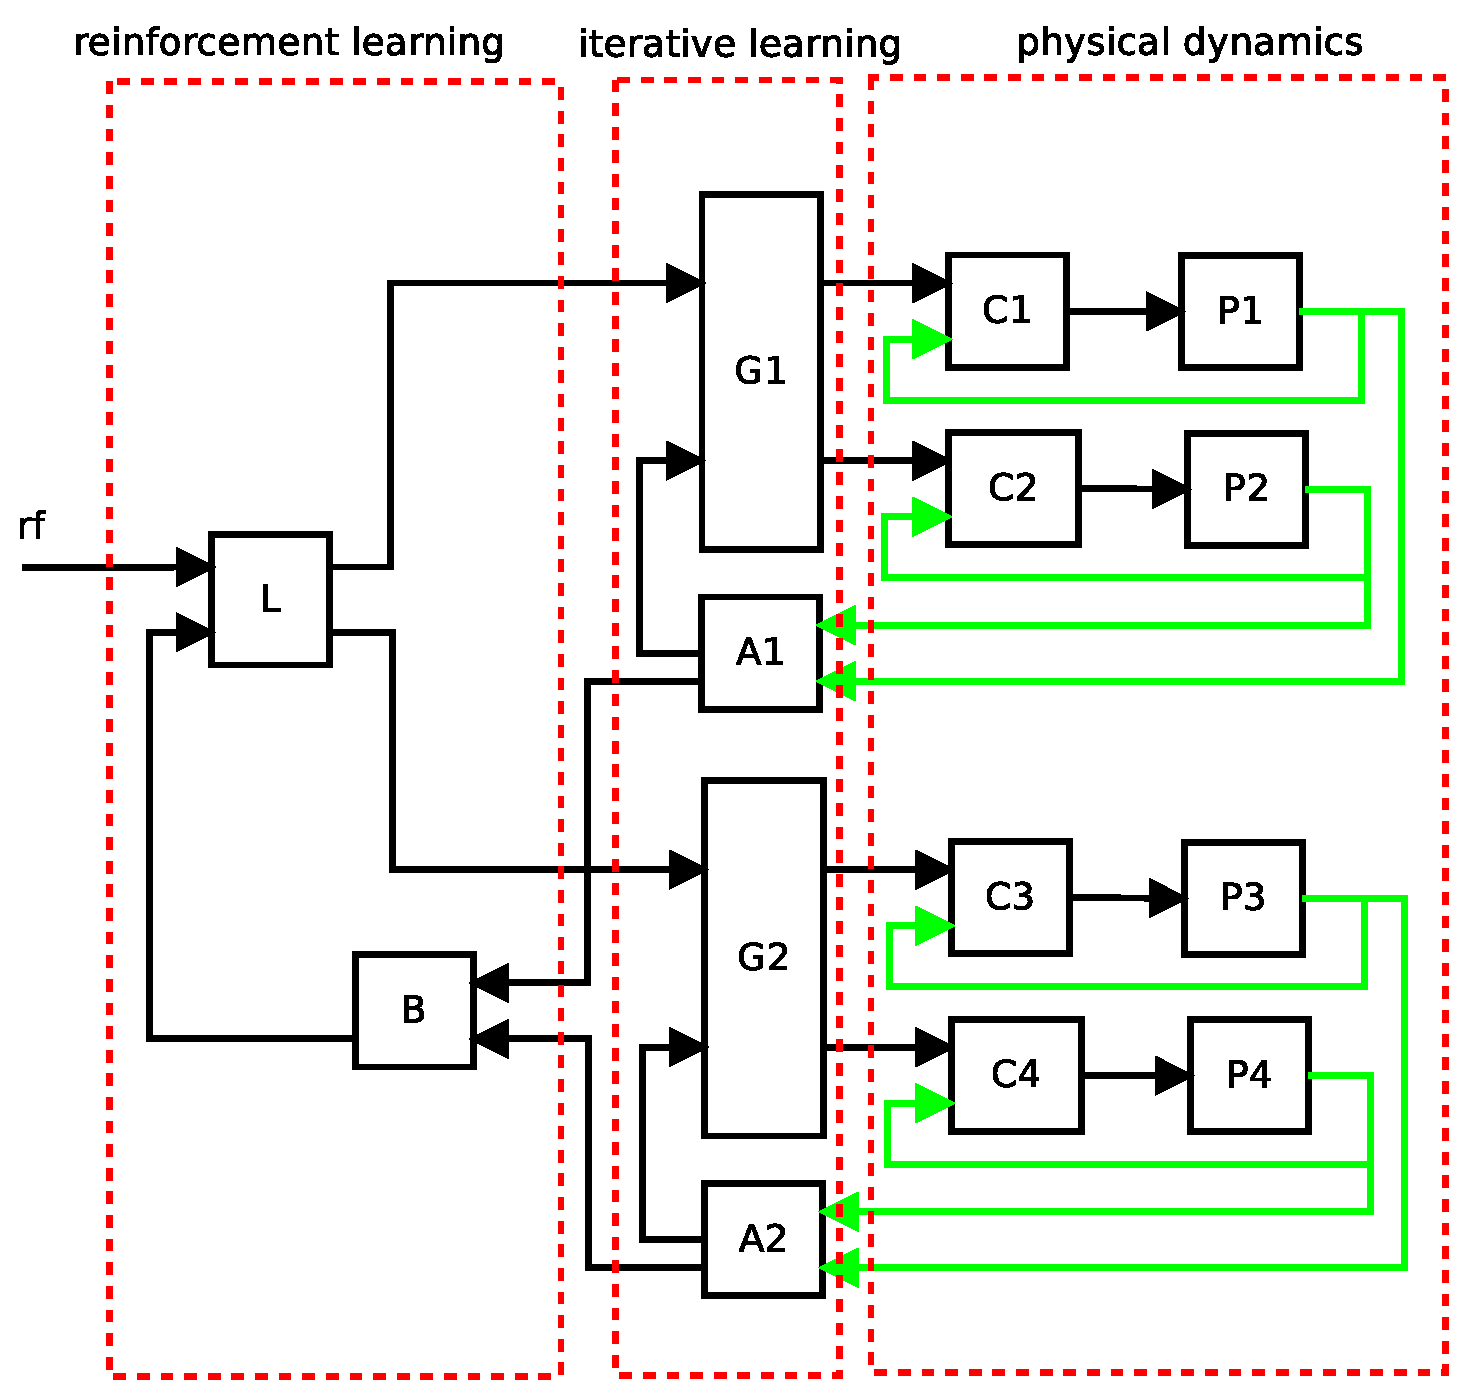
\includegraphics[scale=.5]{../diagrams/hierachical_system.eps}
\caption{Hierarchický systém riadenia}
\label{img:hierachical_controll_system}
\end{figure}

Obrázok je možné vysvetliť na príklade robotického ramena, so 4 stupňami voľnosti.
Cieľom je riadiť 4 sústavy $P1$ až $P4$, Na úrovni fyzikálnej vrstvy je možné použiť
adaptívne PID regulátory, do ktorých vstupuje výstup sústavy a požadovaná hodnota.
V prípade ramena je požadovanou hodnotou natočenie jednotlivých kĺbov. Tieto uhly sú
spočítané blokomi $G1$ a $G2$. Vstupom do regulátorov na fyzikálnej úrovni je tak
postupnosť uhlov generovaná blokomi $G1$ a $G2$. Na tejto úrovni sú zavedené aj
agregačné bloky $A1$ a $A2$, ktoré poskyjú $G$-blokom informáciu o stave systému.
Bloky $G$ spolu s regulátormi $C$ teda úspešne riešenia problém presunu ramena
po zadanej trajektórií.
Veľa systémom to postačuje - operatór výroby ľahko určí požadované trajektórie,
ktoré má robot vykonávať. V prípade komplexného problému, kedy požadované trajektórie
nie sú známe, má zmysel použiť blok $L$ - tretia úroveň, a nechať systém nech si trajektórie
a ich poradie určí sám. Používateľ systému do tohto procesu zasahuje odmeňovaním
alebo trestaním výsledného riešenia. Príkladom môže byť niekoľko kroková montáž výrobku.
Ktoré diely zložiť ako prvé a ktoré ako posledné, aby bol výrobok zložený v čo najkratšom čase

triviálny príklad : osádzanie plošného spoja, osadiť najprv veľké alebo najprv malé súčiastky?
Druhý príklad : V hre šachy je hráč postavený pred rozhodnutie či najprv vybudovať obranu a stratiť niekoľko ťahov,
alebo sa radšej sústrediť na útok a riskovať slabinu vo vlastnej obrane?

V experimentálnej časti bude ako doplnková ukážka uvedený riadiaci mechanizmus robota
Motko Aftermath, sledujúceho čiaru, kde sa požadovaná hodnota určuje predikciou pomocou neurónovej siete a
následne vstupuje do konvenčného regulátora \ref{img:motoko_reloaded}.

\begin{figure}[!htb]
\center
\includegraphics[scale=.1]{../pictures/motoko.jpg}
\caption{Ranná verzia robota}
\label{img:motoko_reloaded}
\end{figure}


\section{Markovove rozhodovacie procesy}


Množstvo úloh je možné popísať množinou stavov $\mathbb{S}$. Pre každý stav je ďalej
definovaná množina akcií $\mathbb{A_S}$ \cite{bib:markov_01} \cite{bib:markov_02}. Pre každý stav a každú akciu, ktorú je v ňom možné vykonať existuje pravedepodobnostná
funkcia prechodu do ďalšieho stavu $P(s, s')$ a za uskutočnené prechody je daná funkcia odmien $R(s, s')$.
Formálne je teda Markovov proces pätica $(\mathbb{S}, \mathbb{A_S}, P(s, s'), R(s, s'), \gamma )$,
kde $\gamma \in (0, 1)$ je faktor zabúdania a volí sa ako parameter procesu. Jeho význam bude vysvetlený
v ďalšej kapitole. Príklad Markovovho rozhodovacieho procesu je na obrázku \ref{img:markovov_decision_process}.
Prechody v grafe znamenajú jednotlivé akcie.

\begin{figure}[!htb]
\center
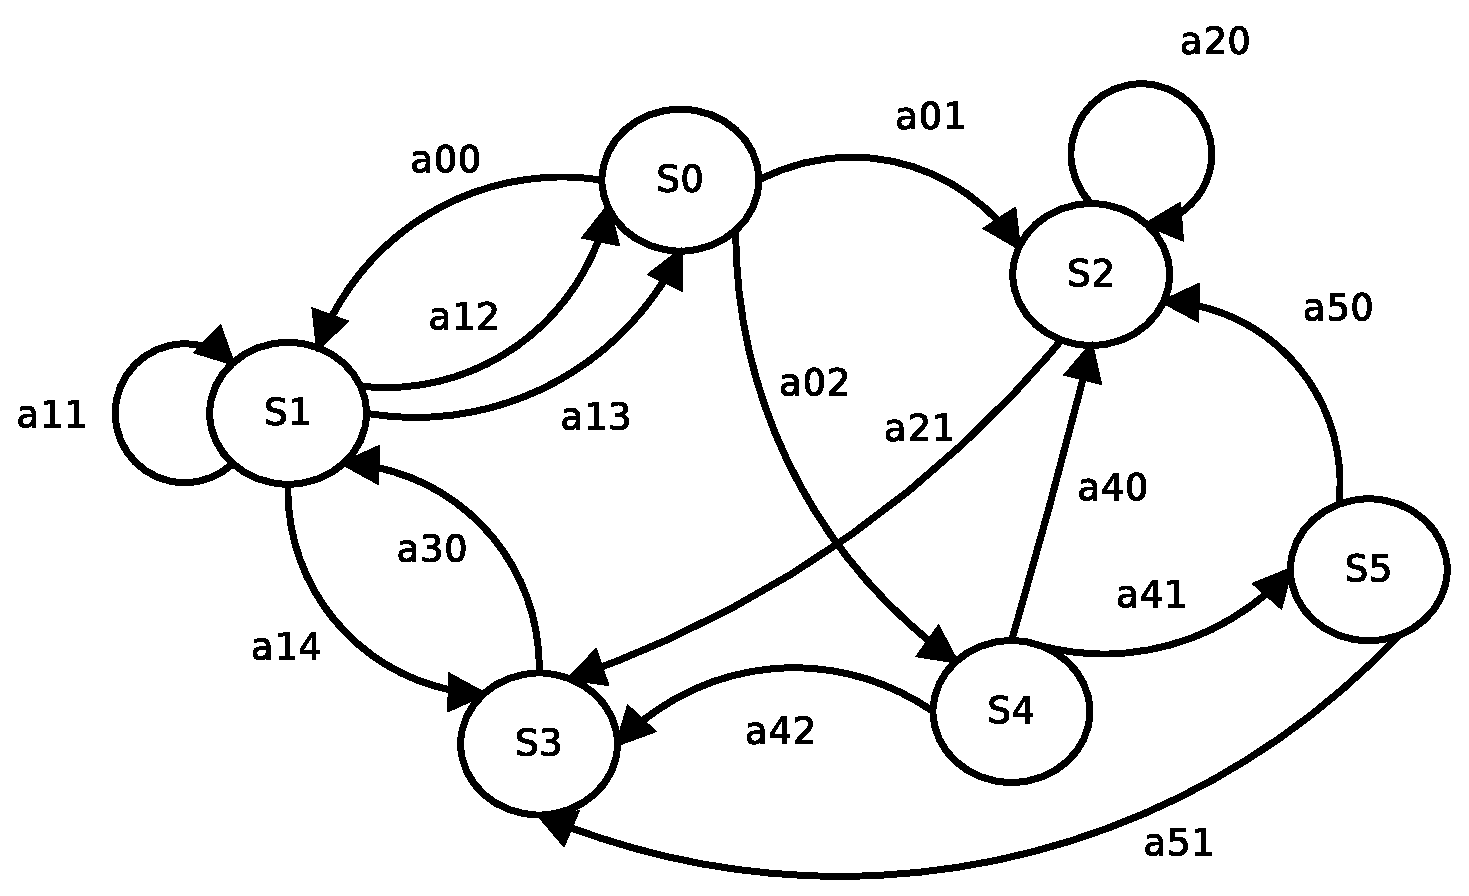
\includegraphics[scale=.5]{../diagrams/markovov_process.eps}
\caption{Markovov rozhodovací proces}
\label{img:markovov_decision_process}
\end{figure}

V priestore stavov $\mathbb{S}$ existuje výkonná jednotka - agent. Je to modul,
ktorý na základe vstupnej informácie - stave vyberie jednu z akcií. To s akou pravdepodobnosťou
sa daná akcia vykoná je dané prostredím (popísané Markovovým rozhodovacím procesom).

Je potrebné poznamenať, že $P(s, s')$ nie je agentovi známa. Agent teda nemôže
vedieť kam sa vykonaním vybranej akcie dostane. Tento fakt značne komplikuje prehľadávanie
priestoru.
Ďalším typickým rysom je, že odmeňovacia funkcia $R(s, s')$, ktorá je zadaná,
nadobúda pre väčšinu prechodov z $s$ do $s'$ hodnotu 0. Je to dôsledok prirodzeného
spôsobu riešenia problémov delením na čiastkové kroky a nie je okamžite známa
veľkosť úžitku po vykonaní čiastkového kroku. Často je táto skutočnosť známa
len pre pár vybraných prechodov.
Dobrým príkladom tejto situácie je hra Go.

\begin{figure}[!htb]
\center
\includegraphics[scale=.5]{../pictures/go2.jpg}
\caption{Hra Go}
\label{img:go_game}
\end{figure}

Položením kameňa na goban nie okamžite známe ako to ovplyvní priebeh hry.
Je bežné, že sa to prejaví až po mnohých krokoch.


\section{Princípy učenia s odmneňovaním}

V systémoch založených na predkladnaní dvojíc vstup - požadovaný výstup
je možné stanoviť chybu a tú vhodnými metódami minimalizovať.
V prípade systému s odmeňovaním sa požaduje od výstupu postupnosť
akcií, ktoré maximalizujú celkovú odmenu.
Príkladom môže byť rozhodovanie robota, ktorý má splniť cieľ pozostávajúci z
niekoľkých elementárnych úkonov, ale postupnosť týchto elementárnych úkonov nie je známa -
nie je teda definovaná požadovaná hodnota výstupu.

Riešením tohto problému je zavedenie systému odmeňovania agenta (robota) \ref{img:reinforcement_learning}.

\begin{figure}[!htb]
\center
\includegraphics[scale=.8]{../diagrams/agent.png}
\caption{Učenie s odmeňovaním}
\label{img:reinforcement_learning}
\end{figure}

Táto metóda sa nazýva  {\bf reinforcement learning}. V súčastnosti predstavuje
najmocnejší nástroj strojového učenia v oblasti umelej inteligencie. Umožňuje
riešiť veľmi komplexné problémy a uplatnenie nachádza nielen v počítačových
hrách, ale napr. aj v robotike.
Jej princíp je možné zhrnúť do týchto bodov :

\begin{enumerate}
  \item Zistenie stavu
  \item Výber akcie
  \item Vykonanie akcie
  \item Prechod do ďalšieho stavu
  \item Získanie odmeny alebo trestu
  \item Učenie sa zo získanej skúsenosti
\end{enumerate}

 {\bf Zistenie stavu} je umožnené vnímaním prostredia, napr. pomocou senzorov.
V najednoduhšom prípade si je možné ako stav predstaviť polohu. Vo
všeobecnosti to ale nemusia byť ani priamo dáta zo vstupov, ale len
príznaky - robot je na križovatke $p_0 = 0.9$, robot je v uličke $p_1 = 0.3$ .
Sada príznakov umožňuje zredukovať dimenziu stavového priestoru (tá musí
byť pre ďalej rozoberané algoritmy konečná, vyplynie to z prezentovaných rovníc).

{\bf Výber akcie} je uskutočnený na základe ohodnotení akcií získanych
v minulosti. Tieto ohodnotenia sú samozrejme závislé od stavu v ktorom sa
systém nachádza - tá ista množina akcií má iné ohodnotenie keď je robot na
križovatke a iné keď je v uličke. Vo fáze prieskumu prostredia môže agent
vyberať tie akcie, ktoré boli v minulosti málo často vykonané, alebo môže vyberať náhodne.
Definovaním veľkosti zmeny ohodnotenia akcie môže uprednostniť tie akcie,
ktorých ohodnotenia vykazujú veľkú zmenu - pretože je pravdepodobné že sa
tým dostane do nepreskúmaných stavov.
Vo fáze kedy agent už nepreskúmavá prostredie, môže vyberať len najlepšie ohodnotenú akciu.
Prípadne môžu existovať v prostredí s viacerími agentami prieskumníci a vykonávatelia.
Navzájom si môžu vymieňať skúsenosti.

{\bf Vykonanie akcie} v deterministickom prostredí sa vybraná akcia vykoná vždy rovnako.
 V nedeterministickom prostredí sa vykonanie sa akcie riadi nejakou pravdepodobnostnou funkciou - napr. robotovi môže prešmyknúť
koleso. Výber agenta vykonať nejakú akciu, teda ešte nutne neznamená že sa táto akcia aj naozaj vykoná.
Táto sutočnosť je daná charakterom prostredia.

{\bf Prechod do ďalšieho stavu} je obvyklým dôsledkom vykonania akcie. Samozrejme, že
v danom stave môže existovať aj taká akcia ktorá nespôsobí zmenu stavu - napr. spomínané
prešmyknutie kolesa - robot sa nepohne.

{\bf Získanie odmeny alebo trestu} po vykonaní akcie, existuje odmeňovací mechanizmus
zadaný tvorcom systému. Preto sa nedá hovoriť o umelej inteligencií - správanie
sa agenta je v deterministickom prostredí plne určené týmto mechanizmom - len nie je známe.
Obvykle platí, že kladné hodnoty dosahuje odmena a záporné trest. Nulová hodnota symbolizuje
neznalosť zadavateľa, a nevie teda určiť či dané konanie bolo dobré alebo zlé.
Nesmierne dôležitý je fakt, že pre veľkú väčšinu rozhodnutí je výsledkom odmeny práve nula.
Príkladom môže byť japonská hra Go - pre úspešné vedenie partie nestačí ohodnotiť
len aktuálny stav na gobane, je potrebné uvažovať viac ťahov dopredu - úspešnosť
ťahu sa často ukáže až po vykonaní množstva ďalších ťahov, kedy je odmena už nenulová.

Práve dominancia nulových odmien je unikátom pre reinforcement learning algoritmy.
Od zadávateľa sa vyžaduje minimum znalostí, je dokonca možné ukázať, že stačí
odmena len v cieľovom stave (i keď proces učenia bude v tomto prípade trvať veľmi dlho).


\section{Ohodnocovanie vykonaných akcií}

Odmena je získaná z prostredia po vykonaní akcie. Ohodnotenie akcie v danom stave
je tvorené predošlými skúsenosťami z vykonania predošlých akcií a získania odmien.
Podstatou učenia je teda ohodnotenie vykonaných akcií v danom stave aby bolo
možné v každom stave rozhodnúť, ktorá akcia je najlepšia - vyberá sa teda
postupnosť akcií $\pi$ pre ktorú je funkcia

\begin{equation}
\Lambda(\pi)  = \sum\limits_{n=0}^{L(\pi)}\gamma^n P_{\pi(n)}(s(n), s(n-1))
\label{eq:q_quality}
\end{equation}

maximálna. Kde $\gamma \in \langle 0, 1 \rangle$ je koeficient zabúdania, $P_{\pi(n)}{(s(n), s(n-1)}$
je odmeňovacia funkcia po prechode zo stavu $s(n-1)$ do stavu $s(n)$ vykonaním $\pi(n)$ a
$L(\pi)$ je dĺžka postupnosti $\pi$

Hľadanie mechanizmu nájdenia maxima $\Lambda(\pi)$ bude vysvetlené na nasledujúcich príkladoch.
Odmena bude známa v každom prechode a je definovaná ako $R(s, a) \in \mathbb{R}$
\\
Pre ilustráciu bude postupnosť prechodov zapísaná priamo ako prameter funkcie $\Lambda$, napr :
$\Lambda(\{S_0, S_7, S_5\})$ predstavuje prechody z $S_0$ do $S_7$ a z $S_7$ do $S_5$.
Ďalej sa predpokladá že $\gamma = 1$.
\\
Je daný systém s troma stavmi, a dvoma prechodmi \ref{img:three_states_system}.
Pre ilustráciu je systém tak jednoduchý, že každá akcia má známu odmenu.

\begin{figure}[!htb]
\centering
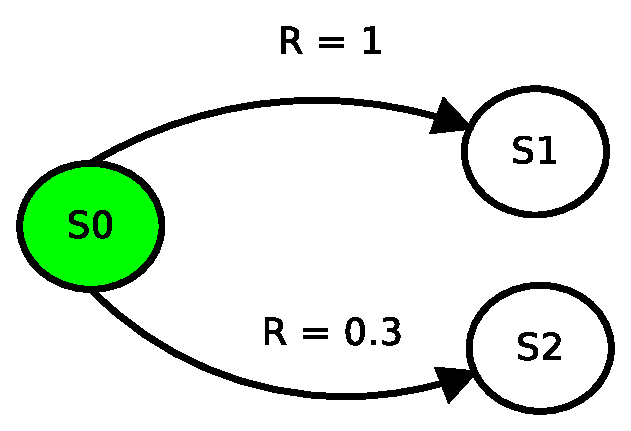
\includegraphics[scale=.6]{../diagrams/rf_two_states.eps}
\caption{Ohodnocovanie akcií v trojstavom systéme}
\label{img:three_states_system}
\end{figure}

V tomto systéme je ohodnotenie $\Lambda(S_a, S_b)$ naozaj triviálne.

\begin{enumerate}
  \item $\Lambda(\{S_0, S_1\}) = 1$
  \item $\Lambda(\{S_0, S_2\}) = 0.3$
\end{enumerate}

Najlepšia cesta je potom $\{S_0, S_1\}$.

V prípade systému s viacerými stavmi \ref{img:multiple_states_system}, ale
známimi ohodnoteniami v každom prechode bude situácia nasledovná.

\begin{figure}[!htb]
\centering
\includegraphics[scale=.6]{../diagrams/rf_more_states.eps}
\caption{Ohodnocovanie vo viacstavovom systéme}
\label{img:multiple_states_system}
\end{figure}

Ohodnotenie ciest :
\begin{enumerate}
  \item $\Lambda(\{S_0, S_1, S_3\}) = 1+(-10) = -9$
  \item $\Lambda(\{S_0, S_1, S_4\}) = 1+3 = 4$
  \item $\Lambda(\{S_0, S_2, S_4\}) = 0.3 +()-1) =-0.7$
  \item $\Lambda(\{S_0, S_1, S_3, S_2, S_4\}) = 1 +(-10) +100 + (-1) = 90$
  \item ...
\end{enumerate}

Jednoduchým ščítaním ohodnotení rôznych ciest je tak možné nájsť optimálnu
postuponosť akcií.

Ak sa v systéme nachádza cyklus \ref{img:cycle_states_system} (na obrázku
je triviálny prípad) potom ohodnotenie bude divergovať. Agent bude mať možnosť
vykonávať akciu, ktorá neustále pripočítava kladnú odmenu, nevyhnutne tak
vyberie túto stratégiu, pretože tak získa nekonečne veľkú odmenu.

\begin{figure}[!htb]
\centering
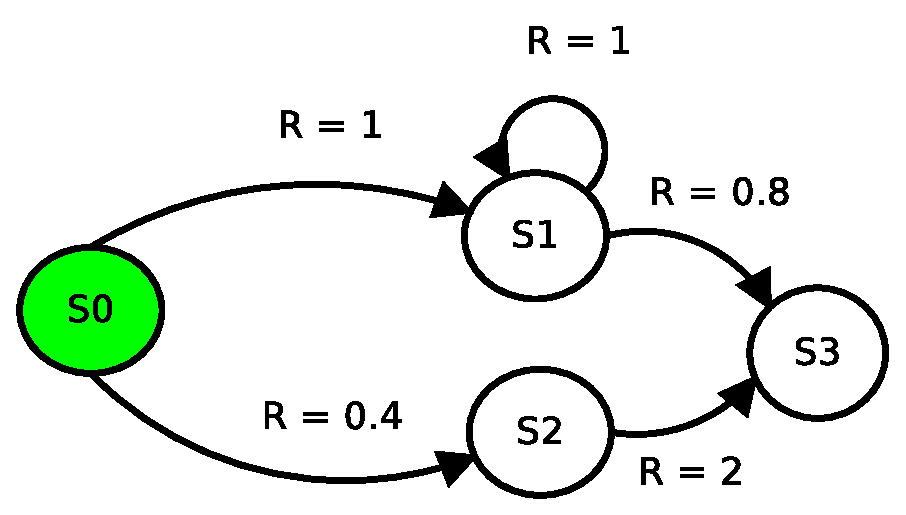
\includegraphics[scale=.6]{../diagrams/rf_cycle_states.eps}
\caption{Ohodnocovanie s cyklom}
\label{img:cycle_states_system}
\end{figure}

Ohodnotenie niektorých ciest :
\begin{enumerate}
  \item $\Lambda(\{S_0, S_2, S_3\}) = 0.4+2 = 2.4$
  \item $\Lambda(\{S_0, S_1, S_3\}) = 1+0.8 = 1.8$
  \item $\Lambda(\{S_0, S_1, S_1, S_1\}) = 1+1+1 = 3$
  \item $\Lambda(\{S_0, S_1, S_1, S_1, S_1\}) = 1+1+1+1 = 4$
  \item $\Lambda(\{S_0, S_1, S_1, S_1, S_1, S_1, ...\}) = 1+1+1+1+1+...+1 = \infty$ !!!!
\end{enumerate}

Riešením je práve zavedenie faktora zabúdania $\gamma$. Ilustračne
bola zvolená $\gamma = 0.9$. Agent tak síce urobí niekoľko cyklov $S_1, S_1$,
po čase ale hodnota odmeny konverguje a minulé príspevky dávajú čoraz menší
a menší úžitok a nevyhnutne tak po niekoľkých cyklov zmení rozhodnutie a prejde
z $S_1$ do $S_3$.

Ohodnotenie niektorých ciest :
\begin{enumerate}
  \item $\Lambda(\{S_0, S_2, S_3\}) = 0.9*0.4 + 2  = 2.36$
  \item $\Lambda(\{S_0, S_1, S_3\}) = 0.9*1 + 0.8 = 1.7$
  \item $\Lambda(\{S_0, S_1, S_1, S_1\}) = 1 + 0.9*(1 + 0.9*1) = 2.71 $
  \item $\Lambda(\{S_0, S_1, S_1, S_1, S_1\}) = 1 + 0.9*(1 + 0.9*(1 + 0.9*1)) = 3.439$
  \item $\Lambda(\{S_0, S_1, S_1, S_1, S_1, S_1, ...\}) = 10$ <-----
  \item $\Lambda(\{S_0, S_1, S_1, S_1, S_1, S_1, ..., S3\}) = 10.8$ <-----
\end{enumerate}

Cyklovanie v $S_1$ teda prinesie celkovú odmenu 10, ale pri prechode do $S_3$ je celková
odmena 11.

Formálny prepis uvedených úvah vedie na Q-learning algoritmus, ktorý zohľadňuje Bellmanov princíp optimality.


\section{Jednostavový systém}

Prv než bude uvedené úplne znenie Q-learning algoritmu je vhodné rozobrať ešte
jeden príklad, a to systém s jedným stavom \ref{img:single_state_system}.
Tento problém vznikol z nasledujúcej úvahy : je daný robot, ktorý má jeden senzor
vzdialenosti od cieľa (nevie teda určiť smer (napr. senzor intenzity osvetlenia) ) a možnosti pohybu o elementárny krok
vpred, vľavo, vpravo, vzad. Ako zvoliť postupnosť akcií aby robot došiel do cieľa - minimalizoval vzdialenosť?
Navyše sa predpokladá, že senzor je nekvalitný a záludný zároveň : poskytuje
informáciu len o tom či sa situácia zlepšila alebo zhoršila (oproti predošlému meraniu),
a s určitou pravdepodobnosťou generuje náhodnú hodnotu - náhodne zmení výsledok (šum).

To vedie na zostavenie odmeňovacej funkcie ako

\begin{equation}
R(n) =
\left\{
	\begin{array}{ll}
		k  & ak \ d(n) - d(n-1) < 0 \\
    -k & inak
	\end{array}
\right.
\label{eq:q_nano_r_func_simple}
\end{equation}

kde $d(n)$ je zmeraná vzdialenosť a na $d(n) - d(n-1) < 0 $ sa pozerá
ako uzavretú časť - vstupon do algoritmu teda nie je samotné $d(n)$ ale až
$R(n)$. Pre $k$ platí

\begin{equation}
k(n) =
\left\{
	\begin{array}{ll}
		-1  & ak \ rnd(0, 1) < p\\
    1 & inak
	\end{array}
\right.
\label{eq:q_nano_r_func_simple_prob}
\end{equation}

kde $p$ je pravdepodobnosť zmeny nameranej hodnoty $p \in \langle 0, 1 \rangle $ a $rnd(0, 1)$ generuje náhodné
číslo z intervalu $\langle 0, 1 \rangle$.

\begin{figure}[!htb]
\centering
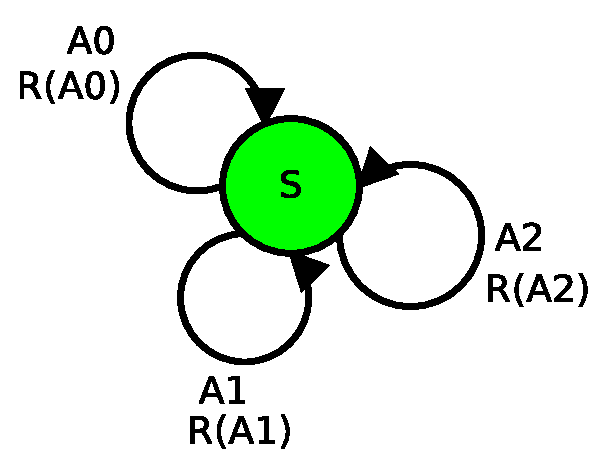
\includegraphics[scale=.6]{../diagrams/single_state.eps}
\caption{Jednostavový systém s troma akciami}
\label{img:single_state_system}
\end{figure}

Kľúčový je výber akcie $a(n)$ z konečnej množiny akcií $\mathbb{A}$,
vychádza sa z predstavy : ak má vykonaná akcia dobré ohodnotenie,
vykoná sa znova, ak má zlé ohodnotenie, vyberie sa iná, náhodná akcia.
Formálne zapísané

\begin{equation}
a(n) =
\left\{
	\begin{array}{ll}
		a(n-1)  & ak \ Q_{n-1}(a(n-1)) > 0 \\
    random(a(n-1)) & inak
	\end{array}
\right.
\label{eq:q_nano_action_selection}
\end{equation}

Samotné $Q$ predstavujúce ohodnotenie sa potom vypočíta ako

\begin{equation}
Q_n(A(n)) = R(n) + \gamma  \max_{a'(n-1) \in \mathbb{A}} Q_{n-1}(a'(n-1))
\label{eq:nano_q_func}
\end{equation}

Algoritmus je teda veľmi jednoduchý a možno ho použit na plánovanie pohybu robota.
Robotovi tak nie je vnútené správanie programátorom, ale sám sa naučí ktoré akcie
vyberať.


\subsection{Výsledky experimentu}

Overenie prebehlo s 32 virtuálnymi robotmi. Cieľom bolo naháňať pohyblivý cieľ,
ktorý sa pohyboval po kružnici s rovnicou

\begin{equation}
  X(n) = (0.7cos(ndt), 0.7sin(ndt))
\label{eq:q_nano_target}
\end{equation}

kde $dt = 0.001$. Roboti mohli vyberať zo 4 akcií ktorými menili svoju polohu
\begin{equation}
\mathbb{A} = ( (0, 1), (0, -1), (1, 0), (-1, 0))
\end{equation}

a zmena poloha $R(n)$ robota pri výbere k-tej akcie je potom

\begin{equation}
  R(n) = R(n-1) + A(k)dt
\label{eq:q_nano_move}
\end{equation}

Počiatočné polohy robotov $R(0)$ boli náhodné.
Celý experiment prebiehal v dvojrozmernom priestore obmedzenom na rozsah
polohy $\langle -1, 1 \rangle$. Metrika vzdialenosti bola Euklidovská.

Po 25000 iteráciach sa počítala priemerná chyba z 32 robotov. Vyšetrovala
sa závislosť tejto chyby od zmeny parametrov $\gamma$ a $p$ (na grafe ako gamma a noise).
Pre vybrané prípady boli exportované aj dráhy prvých 8 robotov.

Prostredie sa tak postupne mení z plne deterministického bez šumu až po hodnotu $0.4$,
čo predstavuje $40\%$ pravdepodobnosť zmeny hodnoty senzora. Graf závislosti priemernej chyby
od parametrov $\gamma$ a $p$ je na obrázku \ref{img:nano_q_summary}.

\begin{figure}[!htb]
\centering
\includegraphics[scale=.4]{../../results_q_learning/nano_q_learning/summary_result_average_error_map.png}
\caption{Priemerná chyba 32 robotov po 25000 iteráciach}
\label{img:nano_q_summary}
\end{figure}

Dráhy robotov pre niektoré zvolené parametre sú uvedené v tabuľke \ref{tab:nano_q}

\begin{center}
  \begin{tabular}{ | c | c || c | c |}
    \hline
    $\gamma$ & $p$ & graf dráhy & graf vývoja chyby \\ \hline
    $0.7$ & $0.0$ & \ref{img:nano_q_result_00_path} & \ref{img:nano_q_result_00_error} \\
    $0.7$ & $0.3$ & \ref{img:nano_q_result_03_path} & \ref{img:nano_q_result_03_error} \\
    $0.0$ & $0.4$ & \ref{img:nano_q_result_04_1_path} & \ref{img:nano_q_result_04_1_error} \\
    $0.7$ & $0.4$ & \ref{img:nano_q_result_04_2_path} & \ref{img:nano_q_result_04_2_error} \\
    $0.9$ & $0.4$ & \ref{img:nano_q_result_04_3_path} & \ref{img:nano_q_result_04_3_error} \\
    $0.98$ & $0.4$ & \ref{img:nano_q_result_04_4_path} & \ref{img:nano_q_result_04_4_error} \\
    \hline
    \end{tabular}
    \captionof{table}{Vybrané parametre experimentu a odkaz na grafické znázornenie výsledku}
    \label{tab:nano_q}
\end{center}

\begin{figure}[!htb]
\centering
\includegraphics[scale=.4]{../../results_q_learning/nano_q_learning/result_00/robot_path.png}
\caption{Dráha robotov pre $\gamma = 0.7 p = 0.0$}
\label{img:nano_q_result_00_path}
\end{figure}

\begin{figure}[!htb]
\centering
\includegraphics[scale=.4]{../../results_q_learning/nano_q_learning/result_00/robot_reward.png}
\caption{Vzdialenosť robotov od cieľa pre $\gamma = 0.7 p = 0.0$}
\label{img:nano_q_result_00_error}
\end{figure}



\begin{figure}[!htb]
\centering
\includegraphics[scale=.4]{../../results_q_learning/nano_q_learning/result_03/robot_path.png}
\caption{Dráha robotov pre $\gamma = 0.7 p = 0.3$}
\label{img:nano_q_result_03_path}
\end{figure}

\begin{figure}[!htb]
\centering
\includegraphics[scale=.4]{../../results_q_learning/nano_q_learning/result_03/robot_reward.png}
\caption{Vzdialenosť robotov od cieľa pre $\gamma = 0.7 p = 0.3$}
\label{img:nano_q_result_03_error}
\end{figure}



\begin{figure}[!htb]
\centering
\includegraphics[scale=.4]{../../results_q_learning/nano_q_learning/result_04_01/robot_path.png}
\caption{Dráha robotov pre $\gamma = 0.0 p = 0.4$}
\label{img:nano_q_result_04_1_path}
\end{figure}

\begin{figure}[!htb]
\centering
\includegraphics[scale=.4]{../../results_q_learning/nano_q_learning/result_04_01/robot_reward.png}
\caption{Vzdialenosť robotov od cieľa pre $\gamma = 0.0 p = 0.4$}
\label{img:nano_q_result_04_1_error}
\end{figure}




\begin{figure}[!htb]
\centering
\includegraphics[scale=.4]{../../results_q_learning/nano_q_learning/result_04_02/robot_path.png}
\caption{Dráha robotov pre $\gamma = 0.7 p = 0.4$}
\label{img:nano_q_result_04_2_path}
\end{figure}

\begin{figure}[!htb]
\centering
\includegraphics[scale=.4]{../../results_q_learning/nano_q_learning/result_04_02/robot_reward.png}
\caption{Vzdialenosť robotov od cieľa pre $\gamma = 0.7 p = 0.4$}
\label{img:nano_q_result_04_2_error}
\end{figure}


\begin{figure}[!htb]
\centering
\includegraphics[scale=.4]{../../results_q_learning/nano_q_learning/result_04_03/robot_path.png}
\caption{Dráha robotov pre $\gamma = 0.9 p = 0.4$}
\label{img:nano_q_result_04_3_path}
\end{figure}

\begin{figure}[!htb]
\centering
\includegraphics[scale=.4]{../../results_q_learning/nano_q_learning/result_04_03/robot_reward.png}
\caption{Vzdialenosť robotov od cieľa pre $\gamma = 0.9 p = 0.4$}
\label{img:nano_q_result_04_3_error}
\end{figure}

\begin{figure}[!htb]
\centering
\includegraphics[scale=.4]{../../results_q_learning/nano_q_learning/result_04_04/robot_path.png}
\caption{Dráha robotov pre $\gamma = 0.98 p = 0.4$}
\label{img:nano_q_result_04_4_path}
\end{figure}

\begin{figure}[!htb]
\centering
\includegraphics[scale=.4]{../../results_q_learning/nano_q_learning/result_04_04/robot_reward.png}
\caption{Vzdialenosť robotov od cieľa pre $\gamma = 0.98 p = 0.4$}
\label{img:nano_q_result_04_4_error}
\end{figure}

Z experimentov je zrejmé, že pre málo zašumené prostrednie nemá hodnota parametra
$\gamma$ veľký význam, obrázky :
\ref{img:nano_q_result_00_path}
\ref{img:nano_q_result_00_error},
\ref{img:nano_q_result_03_path}
\ref{img:nano_q_result_03_error}.

S postupným nárastom šumu však pri nevhodne zvolenej hodnote $\gamma$
roboti vykazujú veľkú chybu. Je preto potrebné náležite zväčšovať
parameter $\gamma$, tento priebeh zlepšovania výsledku zvyšovaním parametra $\gamma$
je zrejmy z obrázkov :
\ref{img:nano_q_result_04_1_path}
\ref{img:nano_q_result_04_1_error},
\ref{img:nano_q_result_04_2_path}
\ref{img:nano_q_result_04_2_error},
\ref{img:nano_q_result_04_3_path}
\ref{img:nano_q_result_04_3_error},
\ref{img:nano_q_result_04_4_path}
\ref{img:nano_q_result_04_4_error}.

Algoritmus bol pomenovaný nanoQ a je pod licenciou GNU GPL dostupný na \cite{bib:nano_q_link}.
Je napísaný v jazyku C len s využitím pevnej rádovej čiarky. To umožňuje jeho implementáciu
aj do menej výkonných mikrokontrolérov, s jadrami napr. Cortex M0 alebo MSP430. Učenie
prebieha v reálnom čase a nevyžaduje veľký výpočtový výkon. Podobne, aj pamäťové nároky rastú
lineárne s počtom akcií. Pre veľký počet akcií je vždy možné použit aproximáciu, ktorá bude rozobratá
v ďalších častiach práce.
